\chapter{Beispielablauf}\label{chap:Workflow}

Im Folgenden wird ein Beispielablauf gezeigt, wie man den TGG-Editor benutzen kann. An simplen Beispielen werden die wichtigsten Funktionen gezeigt. 
Eine Übersicht aller Funktionen ist im Kapitel (\ref{chap:kommandos}) zu finden.

	\section{Projekt anlegen}
	Als erstes muss ein Projekt samt Henshin-Datei angelegt werden.

		\begin{enumerate}
			\item Gehe zu $File \rightarrow New \rightarrow Project... \rightarrow General \rightarrow Project$.
			\item Wähle einen beliebigen Projektnamen (z.B. ''Editor'') und erstelle das Projekt.
		\end{enumerate}
		
		\begin{figure}[h!] %{r}{6cm}
			\centering
			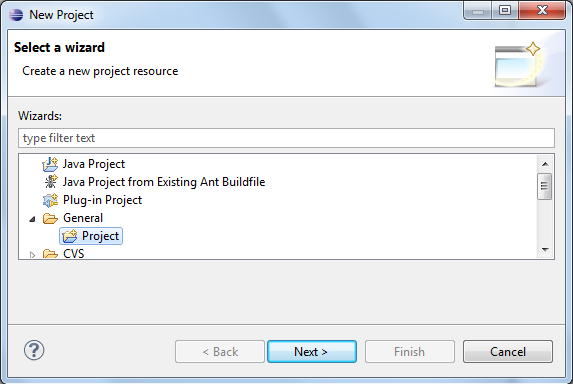
\includegraphics[width=12cm]{workflow/ProjektErstellen}
			\caption{Erstellen eines Standard-Projektes}
			\label{fig:projektErstellen}
		\end{figure}		
		
		Füge nun dem neu erstellen Projekt ein TGG hinzu.
        \begin{enumerate}

			\item[3.] Gehe zu $\rightarrow File \rightarrow New \rightarrow Other... \rightarrow Other \rightarrow TGG\ 			File\ Creation\ Wizard$ 

			\item[4.] Wähle einen beliebigen Namen oder verwende den vorgegebenen. \\ \textcolor{red}		
			{ACHTUNG!} Die Dateiendung muss .henshin bleiben. \\
			Erstelle dann die TGG.
			
			\begin{figure}[h!] %{r}{6cm}
			\centering
			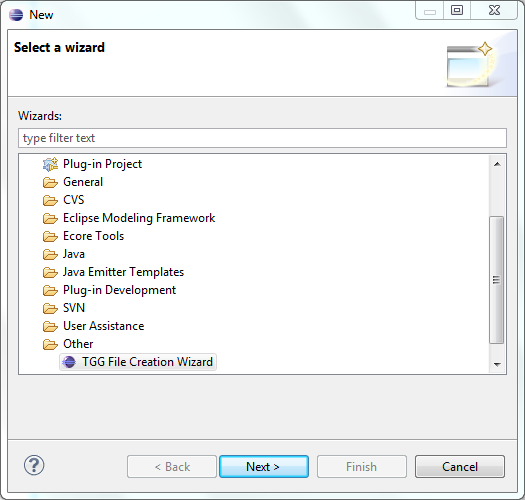
\includegraphics[width=12cm]{workflow/TGGErstellen}
			\caption{Erstellen einer TGG-Datei}
			\label{fig:tggErstellen}
		\end{figure}
		\end{enumerate}

		Mit einem Doppelklick auf das Transformationssystem (im default-Fall heißt es ''Transformation System'') 	
		werden vier Ordner angezeigt, deren Funktionen im Folgenden beschrieben werden.


	\section{EMF Modelle importieren}

	EMF Modelle legen den Graphen zugrundeliegende Strukturen fest. Um einen kompletten Graphen zu erstellen, 
	müssen drei Modelle importiert werden, je eine für Elemente des Source-, des Target- und des Correspondence-
	Bereichs.\\
	\\
	Es wird das Importieren eines Modells beschrieben. Der Import der anderen beiden Modell erfolgt analog.

	\subsection{EMF Projekt importieren}
	Damit der Editor die Referenzen zu dem EMF Modell speichert, muss zuvor noch ein Projekt importiert werden, 
	dass entsprechende Modelle für alle drei Teilgraphen enthält.
		\begin{enumerate}
			\item Gehe zu $File \rightarrow Import \rightarrow Existing\ Projects\ into\ Workspace$
			\item Wähle das EMF Projekt als zip-Archiv oder das Quellverzeichnis des Projekt und importiere das 
			Projekt.
		\end{enumerate}

	\subsection{Import eines EMF Modells}
		\begin{enumerate}
			\item Wähle den Ordner \textit{Imports} und per Rechtsklicks auf den Ordner die Aktion \textit{Import Source}
			\item Wähle über \textit{Workspace...} und das importierte EMF-Projekt, die entsprechende ECORE-Datei für
			 die Source-Komponenten des TGG aus.
		\end{enumerate}
		
		\begin{figure}[h!] %{r}{6cm}
			\centering
			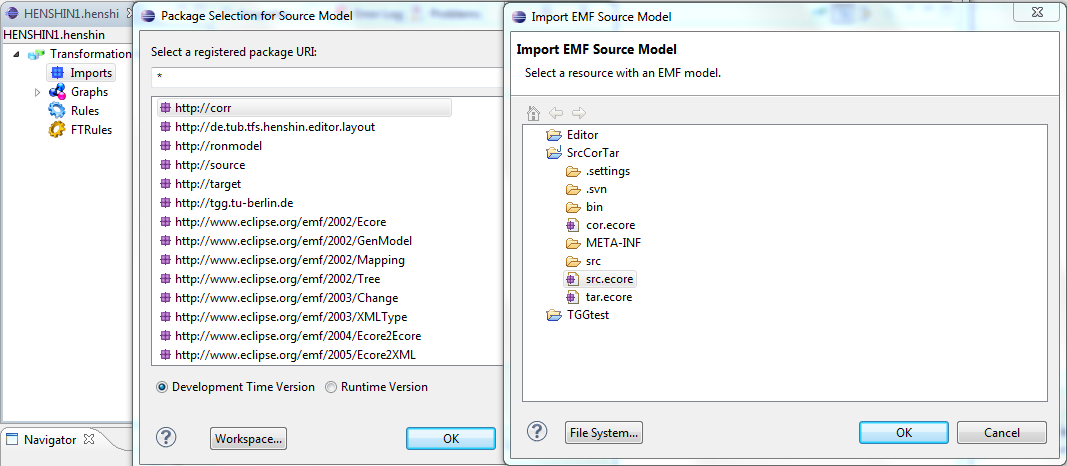
\includegraphics[width=15cm]{workflow/ImportSource}
			\caption{Importieren eines EMF Modells}
			\label{fig:importSource}
		\end{figure}		
		
	Dies muss für Target- und Correspondence-Komponenten wiederholt werden. \\
	Falls aus Versehen eine falsche Datei importiert wurde, kann der Vorgang mit der richtigen Datei wiederholt 
	werden. Danach muss allerdings das Projekt geschlossen und neu geöffnet werden.

	\section{Graphen}
	Nun werden wir einen Graphen erstellen, an dem wir die ersten Editieroperationen zeigen werden.

		\subsection{Einen Graphen erstellen}

			\begin{enumerate}
				\item Öffne über einen Rechtsklick auf den Ordner \textit{Graphs} das Menü und führe die Aktion \textit{Create\ Graph} aus.
				\item Benenne den Graphen in ''GraphExample''.
			
			\begin{figure}[h!]
				\centering
				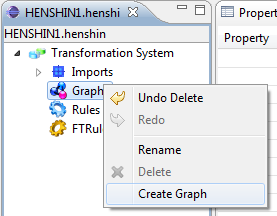
\includegraphics[width=5cm]{workflow/CreateGraph}
				\caption{Erstellen eines Graphen}
				\label{fig:createGraph}
			\end{figure}			
			
			\end{enumerate}
			
		\subsection{Graphen editieren}
		\label{section:graphEditieren}
			\begin{enumerate}
				\item Ein Doppelklick auf den Ordner \textit{Graphs} zeigt alle erstellten Graphen an.

				\item Per Doppelklick auf einen Graphen wird die Ansicht des Graphen geöffnet und man erhält im 
				rechten Rand eine Palette mit diversen Editieroperationen und einigen Aktionen in der Menüleiste 
				des Graphen.
			\end{enumerate}
			
			\subsubsection{Knoten erstellen}
	
			Welche Typen von Knoten erstellt werden dürfen, ist in den EMF Modellen definiert.			
			
			\begin{enumerate}			
				\item Wähle in der Palette das Tool zum Erstellen eines Knoten vom Typ \textit{ClassDiagram} aus.
				
				\item Gehe mit der Maus in den Source-Bereich des Graphen und Erstelle einen Knoten mit einem Linksklick.

			\begin{figure}[h!]%{r}{5cm}
				\centering
				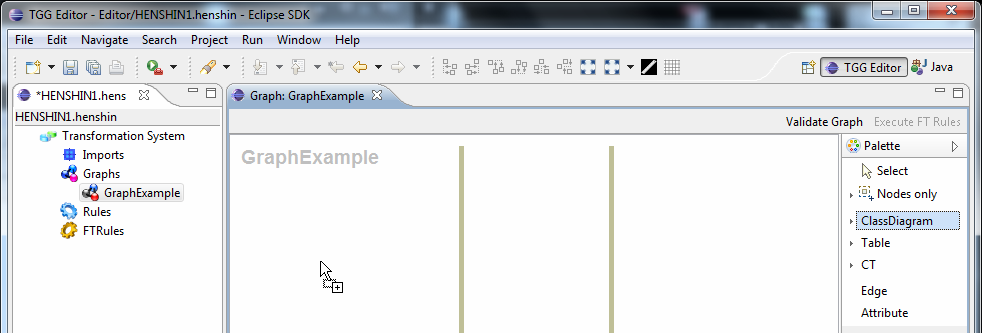
\includegraphics[width=12cm]{workflow/CreateNode}
				\caption{Erstellen eines Knoten}
				\label{fig:createNode}
			\end{figure}

%				Ein selektierter Knoten leuchtet rot auf. Neu erstellte Knoten sind automatisch selektiert. Um einen anderen Knoten zu selektieren, klicke diesen an.

				\item Klicke auf einen selektierten Knoten, um diesen umzubenennen (z.B. ''CD'').
				
				\item erstelle zwei weitere Knoten, einen vom Typen \textit{Database} im Targetbereich und einen vom Typen \textit{CD2DB} im Correspondence-Bereich und benenne den \textit{Database}-Knoten um (z.B. ''DB'').
			\end{enumerate}
						
			\begin{figure}[h!]%{r}{5cm}
				\centering
				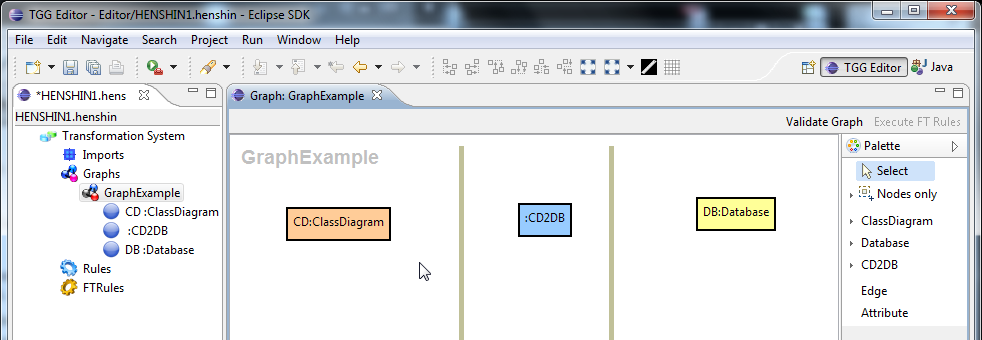
\includegraphics[width=12cm]{workflow/GraphKnotenFertig}
				\caption{Ein Graph mit allen Root-Knoten}
				\label{fig:graphKnotenFertig}
			\end{figure}						
						
			\subsubsection{Kante erstellen}			

			Kanten haben einen Quell- und einen Ziel-Knoten. Kanten werden immer vom Quell- zum Ziel-Knoten gezeichnet.\\
			Es kann vorkommen, dass ein Knotentyp sowohl Ziel- als auch Quellknoten einer Kante sein darf.\\
			Welche Typen von Kanten es gibt, wurde in dem EMF Modellen definiert. 
			
			\begin{enumerate}
				\item Wähle in der Palette das Tool zum Erstellen einer Kante (Edge) aus.
				
				\item Klicke den Knoten \textit{:CD2DB} und danach den Knoten \textit{DB:Database}.
				
			\begin{figure}[h!]%{r}{5cm}
				\centering
				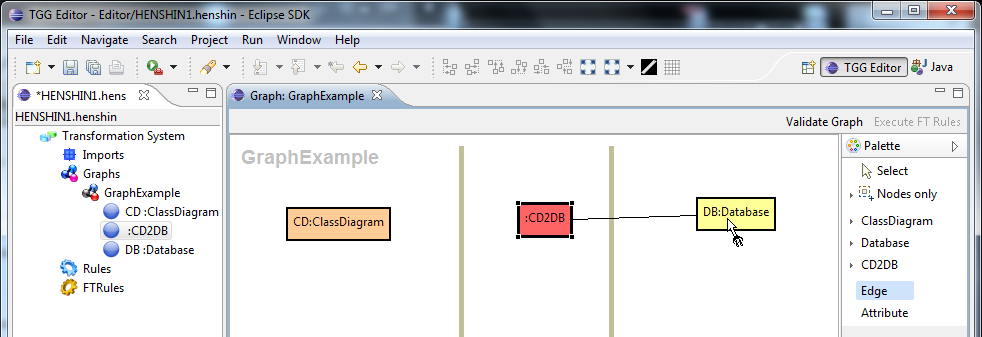
\includegraphics[width=12cm]{workflow/GraphKanteErstellen}
				\caption{Eine Kante zwischen zwei Knoten ziehen}
				\label{fig:graphKanteErstellen}
			\end{figure}				
				
				\item Erstelle eine zweite Kante und ziehe sie vom Knoten \textit{CD2DB} zum Knoten \textit{CD:ClassDiagram}.
				
			\end{enumerate}

			\subsubsection{Attribute erstellen}
			Nicht alle Knoten besitzen Attribute, so z.B. ClassDiagram- und Database-Knoten.\\
			Da an den bisherigen Knoten keine Attribute erstellt werden können, wird diese Operation später noch gezeigt.\\
			Welche Knoten Attribute besitzen und wieviele, ist ebenfalls in dem EMF Modellen definiert.\\
					
	\section{Regeln}
	
	\subsection{Eine Regel erstellen}
	\begin{enumerate}
		\item Über ein Rechtsklick auf den Ordner \textit{Rules} lässt sich die Aktion \textit{Create Rule} ausführen
		\item Wähle einen beliebigen Namen für eine Regel (z.B. ''RuleExample'', der noch nicht vergeben ist.
	\end{enumerate}
	
	\subsection{Eine Regel editieren}
	Die grundlegenden Editieroperationen wurden schon im Kapitel \ref{section:graphEditieren} \nameref{section:graphEditieren}  erklärt.
	Nun werden spezielle Operationen für Regeln erklärt, für die allerdings noch einige Elemente in der Regel erstellt werden müssen, wie es schon für den Graphen gezeigt wurde.
	
		\begin{itemize}
			\item Erstelle dazu eine neue Regel, öffne sie und erstelle alle Elemente aus den Beispielen für den Graphen auch in der Regel.
			\item Erstelle drei weitere Knoten der Typen \textit{Class}, \textit{CT} und \textit{Table}.
			\item Ziehe Kanten zwischen den eben erstellten Knoten ($CT  \longrightarrow Class$ und $CT \longrightarrow Table$).
			\item Erzeuge noch zwei Kanten vom Knoten \textit{CD:ClassDiagram} zum Knoten \textit{:Class} und vom Knoten \textit{DB:Database} zum Knoten \textit{:Table}.
		\end{itemize}
		
		\begin{figure}[h!]%{r}{5cm}
			\centering
			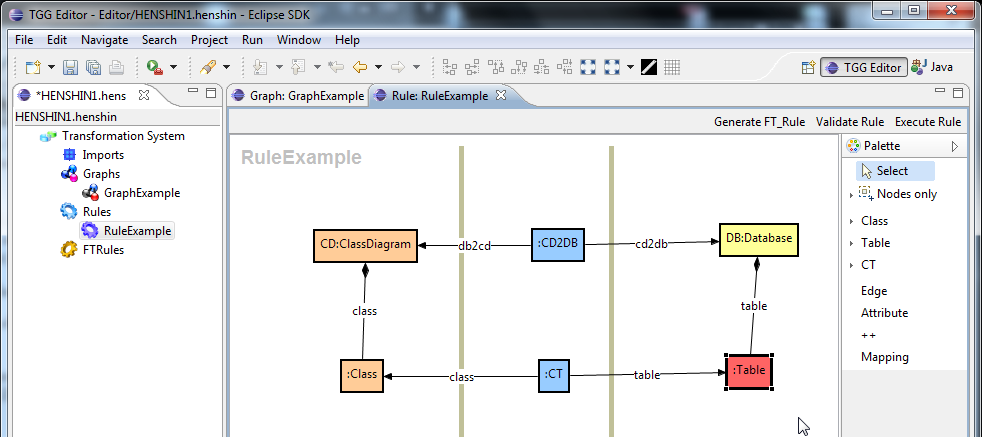
\includegraphics[width=12cm]{workflow/RegelVorNew}
			\caption{Ein Regel ohne als neu markierte Elemente}
			\label{fig:regelVorNew}
		\end{figure}		
			
		\subsubsection{Element als \textit{new} \textcolor{green}{<++>} markieren}
			\begin{enumerate}
				\item Wähle in der Palette das Tool \textit{++} um ein Element als neu zu markieren.
				\item Klick auf die Knoten \textit{:Class}, \textit{:CT} und \textit{:Table}.
			\end{enumerate}
			
			\begin{figure}[h!]%{r}{5cm}
				\centering
				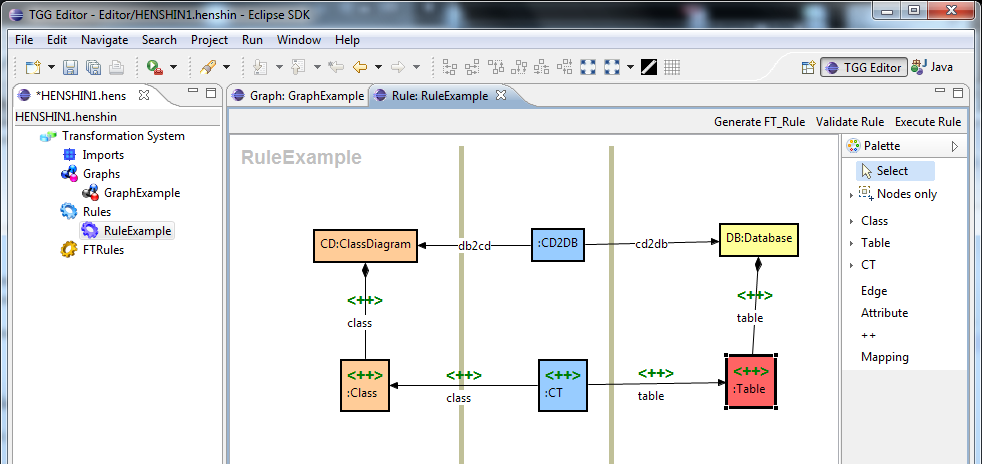
\includegraphics[width=12cm]{workflow/RegelKnotenNeu}
				\caption{Eine Regel, die Elemente neu erzeugt}
				\label{fig:regelKnotenNeu}
			\end{figure}
					
		Hinweise: 
		\begin{itemize}
			\item Markiert man einen Knoten mit \textcolor{green}{<++>}, werden alle anhängenden Kanten ebenfalls markiert.
			\item Demarkiert man einen Knoten werden alle Kanten ebenfalls demarkiert, es sei denn, der andere Knoten der Kante ist noch mit \textcolor{green}{<++>} markiert.
			\item Kanten können einzeln de-/markiert werden.
		\end{itemize}
		
		\subsubsection{Parameter erstellen}		
			\begin{enumerate}
				\item Wähle in der Baumansicht die Regel ''RuleExample'' aus.
				\item Aktiviere per Linksklick lässt sich die Aktion \textit{Create Parameter}.
				\item Gib dem Parameter einen Namen (z.B. ''cn'').
			\end{enumerate}
			
		\subsubsection{Attribute erstellen}
			\begin{enumerate}
				\item Wähle das Toole \textit{Attribute} in der Palette und klicke auf den Knoten \textit{:Table}.
				\item Suche das Attribute \textit{name} aus und gib ihm den Wert 'tablename'.
				\item Füge dem Knoten \textit{:Class} ein Attribute hinzu und nenne es cn (ohne die '').
			\end{enumerate}
			\begin{figure}[h!]
			    \subfigure[Den Wert eines Attributs sofort setzen]{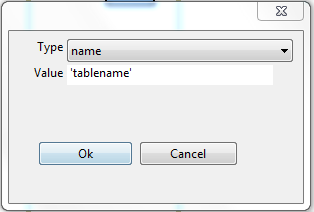
\includegraphics[width=0.4\textwidth]{workflow/AttributeErstellen}}
			    \hfill
			    \subfigure[Den Wert eines Attributs über einen Parameter setzen]{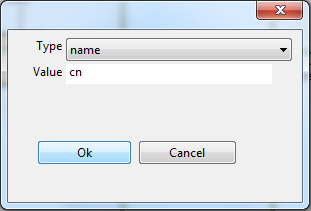
\includegraphics[width=0.4\textwidth]{workflow/AttributeErstellen2}}
				\caption{Attribute erstellen}
			\end{figure} 

			\begin{figure}[h!] %{r}{6cm}
				\centering
				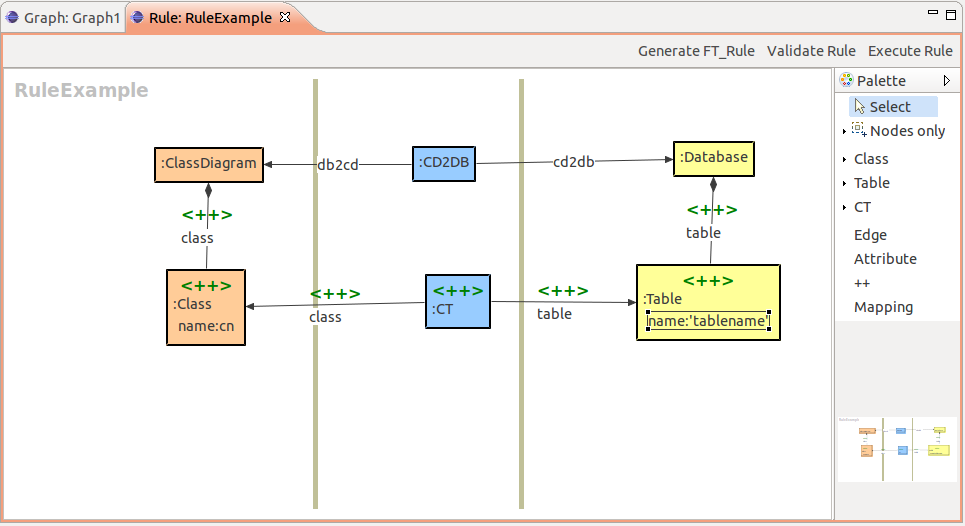
\includegraphics[width=12cm]{workflow/RegelFertig}
				\caption{Eine gültige Regel}
				\label{fig:regelFertig}
			\end{figure}

		\subsubsection{NAC erstellen}
			\begin{enumerate}
				\item Öffne das Menü der Regel ''RuleExample'' und führe die Aktion \textit{Create NAC} aus und benenne die NAC 'NAC1'.
				\item Schließe die Regel ''RuleExample'' und öffne sie wieder. Jetzt erscheint die NAC in der Editor-View.
			\end{enumerate}
		
		\subsubsection{NAC editieren}
		Das Editieren einer NAC läuft nach dem gleichen Schema wie das Editieren eines Graphen ab. Siehe dazu \ref{section:graphEditieren} \nameref{section:graphEditieren}.\\
		Erstelle in der NAC einen Knoten vom Typ \textit{Class}.
				
		\subsubsection{NAC-Mapping erstellen}
			\begin{enumerate}
				\item Erstelle einen weiteren Knoten vom Typ \textit{Class} in der Regel und benenne ihn ''A''.
				\item Wähle in der Palette das Tool \textit{Mapping} aus.
				\item Markiere den \textit{:Class}-Knoten in der Regel als Quell-Knoten des Mappings.
				\item Markiere den Knoten aus der NAC als Ziel-Knoten.
			\end{enumerate}
		
			Wie in \autoref{fig:nacMapping} ''\nameref{fig:nacMapping}'' abgebildet, werden NAC-Mappings durch eine simple Nummerierung angezeigt. Die Nummerierung geschieht automatisch nach dem Index des Knotens in der Liste aller Knoten im Graphen.
			
			\begin{figure}[h!] %{r}{6cm}
				\centering
				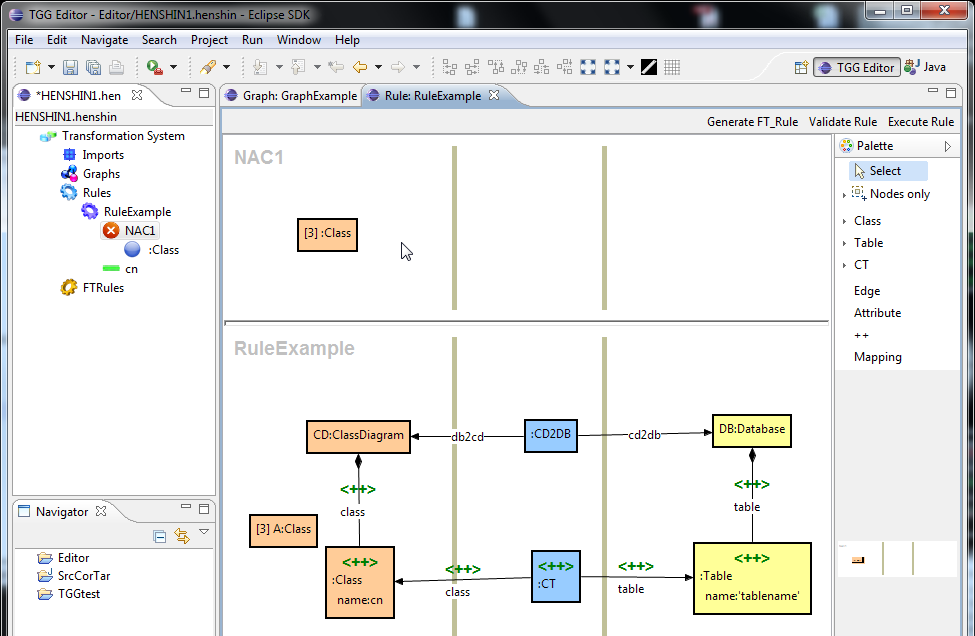
\includegraphics[width=12cm]{workflow/NACMapping}
				\caption{Ansicht einer Regel mit einem NAC-Mapping}
				\label{fig:nacMapping}
			\end{figure}
			
		\subsubsection{NAC-Mapping löschen}	
		\begin{enumerate}
			\item Selektiere den NAC-Knoten führe über das Menü die Aktion \textit{Delete NAC Mappings} aus.
		\end{enumerate}
		
		\subsubsection{Knoten löschen}
		\begin{enumerate}
			\item Selektiere den Knoten \textit{A:Class} und führe über das Menü die Aktion \textit{Delete} aus.
		\end{enumerate}

		\subsubsection{NAC löschen}
		\begin{enumerate}
			\item Selektiere die NAC der Regel in der Baumansicht und führe über das Menü die Aktion \textit{Delete} aus.
			\item Schließe und öffne die Regel neu, damit die Ansicht aktualisiert wird.
		\end{enumerate}
		
		Sie sollte nun wieder so aussehen, wie in \autoref{fig:regelFertig} \nameref{fig:regelFertig} gezeigt.
		
	\section{Forward-Translation-Regeln}
	
	\subsection{FT\_Regel generieren}
		\begin{enumerate}
			\item Öffne die Regel "RuleExample".
			\item Klicke in der Menüleiste der Regel den Button \textit{Generate FT\_Rule}.
		\end{enumerate}
	
			\begin{figure}[h!] %{r}{6cm}
				\centering
				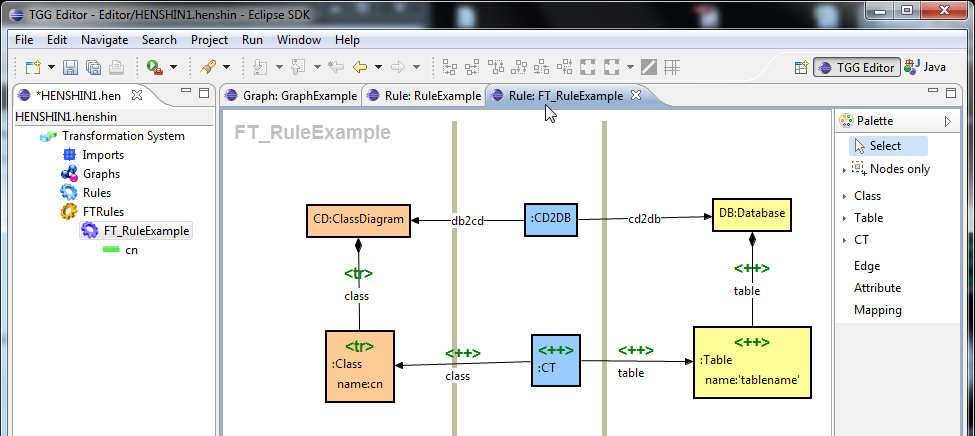
\includegraphics[width=12cm]{workflow/FT_Regel}
				\caption{Ansicht einer FT\_Regel}
				\label{fig:ft_Regel}
			\end{figure}	
	
	\subsection{FT\_Regel editieren}
	Es wird nur gestattet, die NACs einer FT\_Regel zu editieren (siehe NAC editieren) sowie die NAC-Mappings zwischen der FT\_Regel und deren NACs.\\
	Um Änderungen an einer FT\_Regel vorzunehmen, muss die entsprechende Regel geändert werden und daraus dann eine neue FT\_Regel generiert werden (vorhandene FT\_Regeln werden in diesem Fall überschrieben).
	
	\section{Regeln Ausführen}
	
		\subsection{Graph validieren}	
		Um eine Regel ausführen zu können, muss der Graph auf dem die Regel ausgeführt werden soll, valide sein.
		
		\begin{enumerate}
			\item Öffne den Graphen ''GraphExample''.
			\item Klicke den Button \textit{Validate Graph}.
			\item Es erscheint eine Erfolgsmeldung, wenn alles korrekt war. Editiere den Graphen ggf. entsprechend der Hinweise, falls Fehler aufgetreten sind.
		\end{enumerate}
		
		\subsection{Regel validieren}
		Eine Regel muss ebenfalls valide sein.
		
		\begin{enumerate}
			\item Öffne den Graphen ''RuleExample''.
			\item Klicke den Button \textit{Validate Rule}.
			\item Es erscheint eine Erfolgsmeldung, wenn alles korrekt war. Editiere die Regel ggf. entsprechend der Hinweise, falls Fehler aufgetreten sind.
		\end{enumerate}
	
		\subsection{Regel ausführen}
		\begin{enumerate}
			\item Öffne die Regel ''RuleExample'' und klicke den Button \textit{Execute Rule}.
			\item Setze den Wert des Parameters auf 'classname'.
		\end{enumerate}
			\begin{figure}[h!] %{r}{6cm}
				\centering
				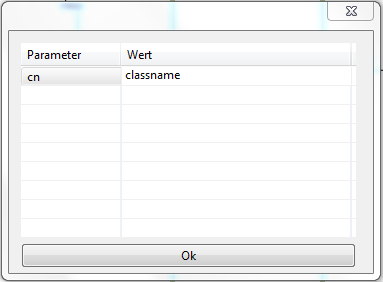
\includegraphics[width=7cm]{workflow/RegelAusfuehrenParaSetzen}
				\caption{Das Setzen eines Parameterwertes beim Ausführen einer Regel}
				\label{fig:regelAusfuehrenParaSetzen}
			\end{figure}	

		\begin{enumerate}					
			
			\item[3.] Öffne anschließend den Graphen ''GraphExample''.
		\end{enumerate}
		
		Alle Elemente, die in der Regel mit \textcolor{green}{<++>} markiert wurden, sind in dem Graphen neu erstellt worden.
		
		\subsection{FT\_Regel ausführen}
		\begin{enumerate}
			\item Erstelle eine neue Regel, die Knoten von Typ \textit{ClassDiagram}, \textit{CD2DB} und \textit{Database} sowie Kanten vom Typ \textit{db2cd} und \textit{cd2db} neu erstellt und generiere dazu eine FT\_Regel.
			\item Löschen in dem Graphen ''GraphExample'' alle Elemente die nicht zum Source-Bereich des Graphen gehören.
		
		\end{enumerate}
			\begin{figure}[h!] %{r}{6cm}
				\centering
				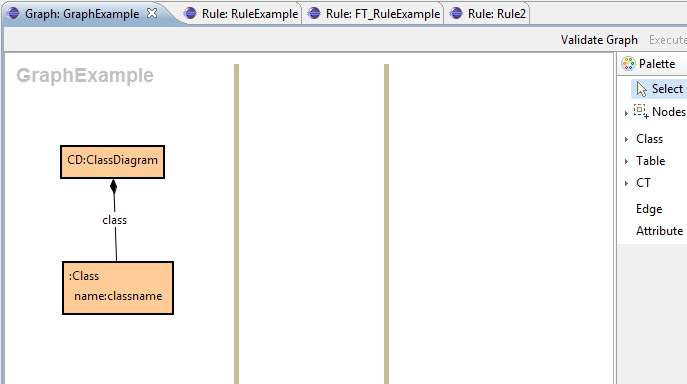
\includegraphics[width=12cm]{workflow/GraphFuerFTRegel}
				\caption{Aussehen eines Graphen für die Ausführung der FT\_Regeln}
				\label{fig:graphFuerFTRegel}
			\end{figure}	
		\begin{enumerate}
			\item[3.] Öffne das Menü des Graphen in der Baumansicht und führe die Aktion \textit{Execute FT\_Rules} aus
		\end{enumerate}
